\section{Nuclear Transparency}

\begin{equation}
    T(Q^2) = \frac{\int_{V} d^{3} p_{m} d E_{m} Y_{exp }(E_{m}, \vec{p}_{m})}
                  {\int_{V} d^{3} p_{m} d E_{m} Y_{PWIA}(E_{m}, \vec{p}_{m})}
\end{equation}


% TODO: replace this with a pdf
\begin{figure}[!h]
    \centering
    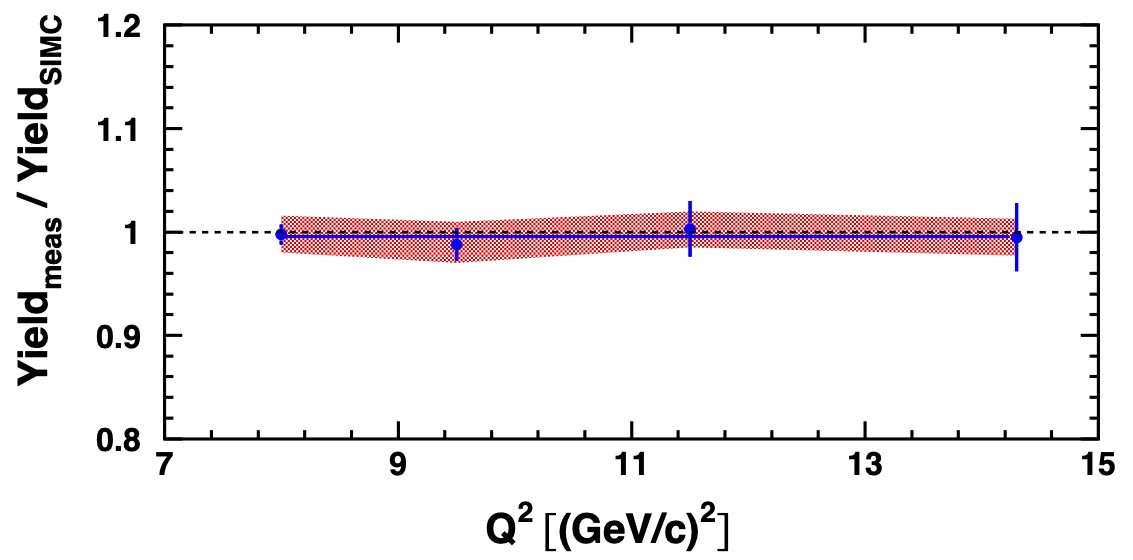
\includegraphics[width=0.8\textwidth]{chap5/lh2_results.png}
    \caption{
            Nuclear transparency for ${}^{1}H(e,e'p)$ as a function of
            momentum transfer.
            The error bars represent statistical uncertainty and the
            shaded band represents the 4.0\% systematic uncertainty.
            }
    \label{fig:lh2_transparency_results}
\end{figure}



\begin{figure}[!h]
    \centering
    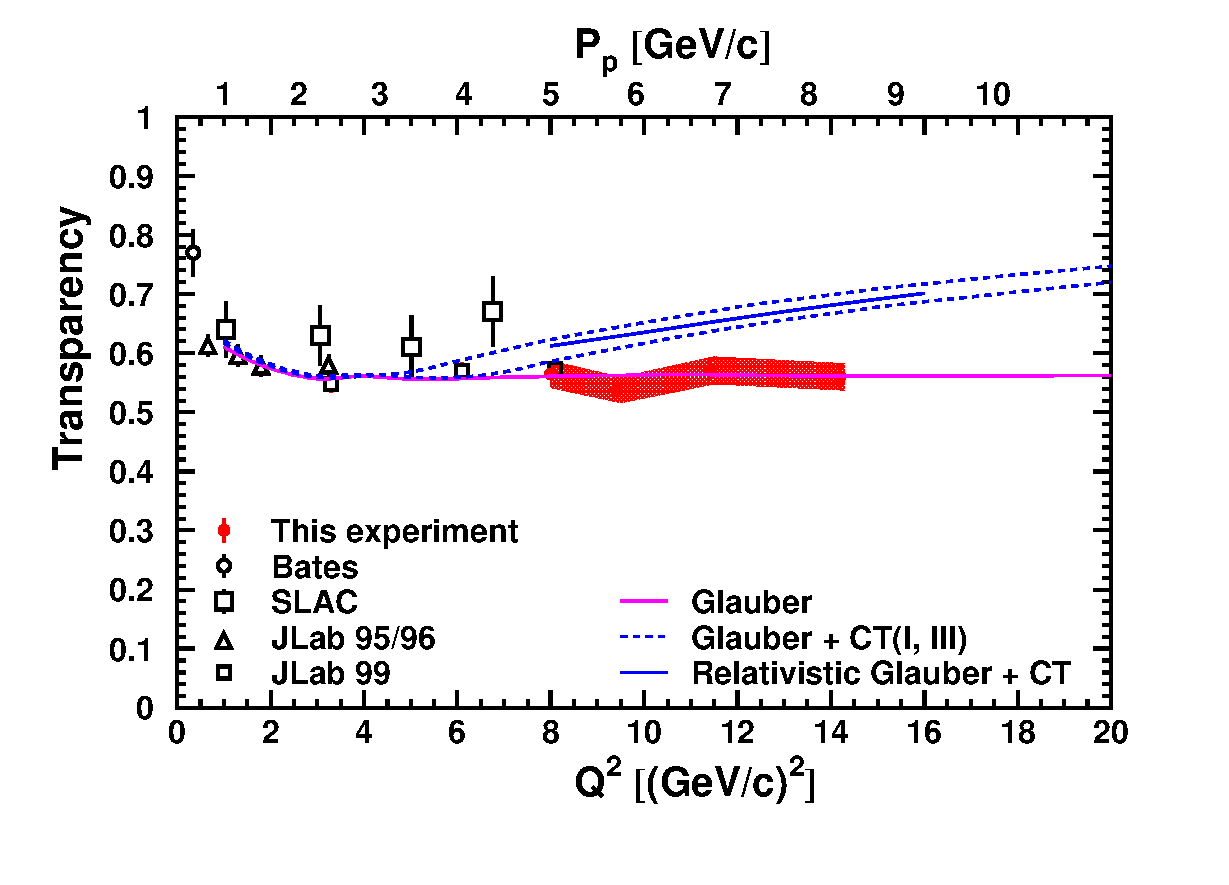
\includegraphics[width=0.8\textwidth]{chap5/c12_results.pdf}
    \caption{
            Nuclear transparency for ${}^{12}C(e,e'p)$ as a function of
            momentum transfer.
            The results of this experiment, E12-06-107, are shown in red along
            with previous measurements in open shapes.
            The error bars represent statistical uncertainty and the
            shaded band represents the 4.0\% systematic uncertainty.
            The magenta line is the prediction of a Glauber
            model that does not include CT~\cite{Pandharipande_1992}.
            The dashed lines represent predictions, for two choices of
            parameters, of a model including CT~\cite{Frankfurt_1995_PRC}.
            The solid line represents the prediction of a relativistic Glauber
            model that includes CT~\cite{Cosyn_2006}.
            }
    \label{fig:c12_transparency_results}
\end{figure}

\subsection{Statistical Uncertainty}

\subsection{Systematic Uncertainty}

Table~\ref{tab:systematic_uncertainty} lists the major sources of systematic
uncertainty in our measurements of nuclear transparency.
The systematic uncertainty due to spectrometer acceptance was estimated by
taking the average of the bin-wise difference between the normalized missing
momentum spectra for data and simulation.

\begin{table}[htb!]
    \caption{
        Systematic uncertainties in our measurements of nuclear
        transparency.
        $Q^2$-dependent uncertainties are averaged over all kinematic settings.
        The total uncertainty is the quadrature sum of the individual
        contributions.
    }
    \label{tab:systematic_uncertainty}
    \centering
    \begin{tabular}{lc}
        \hline
        \hline
        Source                            & $Q^2$-dependent uncertainty (\%) \\
        \hline
        Spectrometer acceptance           & 2.6                              \\
        Event selection                   & 1.4                              \\
        Tracking efficiency               & 0.5                              \\
        Radiative corrections             & 1.0                              \\
        Live time \& detector efficiency  & 0.5                              \\
        \hline
        \hline
        Source                            & Normalization uncertainty (\%)   \\
        \hline
        Free cross section                & 1.8                              \\
        Target thickness                  & 0.5                              \\
        Beam charge                       & 1.0                              \\
        Proton absorption                 & 1.2                              \\
        \hline
        \hline
        Total                             & 4.0                              \\
    \end{tabular}
\end{table}

The uncertainty in the spectral function includes the effects of the off-shell
$\sigma_{ep}$ of 2\%, the electric and magnetic form factors of the proton (2\%)
as previously determined\,\cite{ONeill_1995}.
